\documentclass{article} % For LaTeX2e
\usepackage[a4paper,margin=1.5in]{geometry}
\usepackage[mathlines]{lineno}
\usepackage{hyperref}
\usepackage{url}
\usepackage{amsmath}
\usepackage{graphicx}
\usepackage{bm}
\usepackage{hyperref}
\usepackage{natbib}
\usepackage{latexsym,amsbsy,amssymb,color,xspace, booktabs}

\include{macros}
\newcommand{\entropy}{\calH}

\newcommand{\sigmak}{\sigma_{k}}
\newcommand{\der}{\mathrm{d}}

\newcommand{\sigmanoise}{\sigma_{\text{n}}}
\newcommand{\sigmoid}{\text{sig}}
\newcommand{\Xu}{\mat{X}_u}
\newcommand{\bs}{\boldsymbol}
\newcommand{\xstar}{x_*}
\newcommand{\fstar}{f_*}
\newcommand{\ystar}{y_*}
\newcommand{\zstar}{z_*}
\newcommand{\vxstar}{\x_*}
\newcommand{\vfstar}{\f_*}
\newcommand{\Xuk}{\Xu^{(k)}}
\newcommand{\Kab}[2]{\mat{K}_{\vec{#1},\vec{#2}}}

% model specification
\newcommand{\BigMu}{\bs{\mu}}
\newcommand{\BigSigma}{\mat{\Sigma}}
\newcommand{\Mu}{\BigMu}
\newcommand{\Muk}{\bs{\mu}_k}
\newcommand{\Sigmak}{\mat{\Sigma}_k}
\newcommand{\hatMuk}{\bs{\hat \mu}_k}
\newcommand{\hatSigmak}{\mat{\hat \Sigma}_k}
\newcommand{\hatMukprime}{\bs{\hat \mu}_{k'}}
\newcommand{\hatSigmakprime}{\mat{\hat \Sigma}_{k'}}
\newcommand{\thetak}{\bs{\theta}_k}
\newcommand{\BigTheta}{\bs{\theta}}
\newcommand{\bsigma}{\bs{\sigma}}
\newcommand{\map}{\text{\sc{map}}}
\newcommand{\zmap}{\vz_\text{\sc{map}}}
\newcommand{\fuk}{\vec{g}_k}
\newcommand{\fu}{\vec{g}}
\newcommand{\kernelk}{k^{\BigTheta_k}}
\newcommand{\matUk}{\mat{U}_k}
\newcommand{\matXk}{\mat{X}_k}
\newcommand{\Lambdak}{\Lambda^{\BigTheta_k}}
\newcommand{\matK}{\mat{K}}
\newcommand{\matLambdak}{\mat{\Lambda}_k}

% variational inference
\newcommand{\Mufk}{\BigMu_k}
\newcommand{\Sigmafk}{\BigSigma_k}
\newcommand{\Kuk}{\matK^{(k)}_{\vu,\vu}}
\newcommand{\Psik}{\mat{\Psi}_k}
\newcommand{\Gammak}{\mat{\Gamma}_k}

\def\linenumberfont{\normalfont\small\sffamily}

\title{Multiple Output Regression}

\newcommand{\fix}{\marginpar{FIX}}
\newcommand{\new}{\marginpar{NEW}}

%\nipsfinalcopy % Uncomment for camera-ready version

\begin{document}
\maketitle
\linenumbers

\section{Model Description}
We describe a multiple-output regression model.
Suppose that we have inputs $\X = \{\x_n\}_{n=1}^N$ and outputs $\y = \{\y_n\}_{n=1}^N$, with $\x_n \in \calR^D$ and $\y_n \in \calR^P$, i.e. the output is $P$-dimensional.
For ease of exposition, we assume that there are no missing values in any output dimension.
The most dominant approach in GP-based multiple output regression is to compose the different outputs as some \textit{linear} mixing (combination) of some basic processes (random functions).
Our model is also underpinned by this composition approach.
However, to really address the issue of scalability, this model is built upon sparse GPs from the ground up.


\subsection{Prior and Likelihood}
We use a simple composition:
\begin{align}
f_i(\x) = w_i g(\x) + h_i(\x), \quad i = 1 \hdots P,
\end{align}
where each (latent) output is the sum of two functions: one scaled latent function that is shared by all outputs and one latent function unique to the output.
This allows the outputs to be correlated via the shared function $g(\x)$ while still having their own independent processes.
Furthermore we assume that $g(\x) \sim \GP(0, k_g(\x,\x'; \vectheta_g))$ and $h_i(\x) \sim \GP(0, k_i(\x,\x'; \vectheta_i))$, and that $h_i$ are independent GPs with their own set of hyperparameters. \\

\noindent The auto-variance of the latent output using this composition is
\begin{align}
\nonumber
cov[f_i(\x), f_i(\x')] 
&= cov \left[ \left(w_i g(\x) + h_i(\x) \right) \left(w_{i} g(\x') + h_i(\x') \right) \right] \\
&= w_i^2 k_g(\x, \x') + k_i(\x,\x').
\end{align}
\\
\noindent The cross-covariance of the latent outputs is
\begin{align}
\nonumber
cov[f_i(\x), f_{i'}(\x')] 
&= cov \left[ \left(w_i g(\x) + h_i(\x) \right) \left(w_{i'} g(\x') + h_{i'}(\x') \right) \right] \\
&= w_i w_{i'} k_g(\x, \x').
\end{align} 

\noindent It can be seen that the induced covariance function of $f_i(\x)$ is very similar to that in the MTGP model.
Specifically, in MTGP the task-correlation matrix is a free-form positive definite matrix $B$ whereas here it is the matrix $\w \w^T$ where $\w = [w_1, \hdots, w_P]^T$.
However this model is more flexible compared to MTGP because each output is also influenced by its own independent process $h_i(\x)$.
Note that we can also use more than one shared function $g(\x)$, in which case it becomes the semiparametric latent force model (SLFM), again with the addition of independent process in each output dimension. \\

\noindent 
\textbf{Augmented sparse GPs}
Toward scalable modeling, we replace standard GPs with sparse GPs augmented with \textit{different} set of inducing inputs.
This adds much flexibility to the model as the roles of $g(\x)$ and $h_i(\x)$ can be quite different, so it is necessary that each has its own inducing inputs.
Furthermore, $g(\x)$ can be seen as a \textit{global} function operating on the entire input space (of all output dimensions), while each $h_i(\x)$ operates only on the inputs of the $i$-th output, which can be smaller than that of $g(\x)$.
If more than one $g(\x)$ is used, each $g(\x)$ may capture a different pattern so they should also have separate inducing inputs. \\

\noindent
\textbf{Prior}
\newcommand{\Zg}{\Z_g}
\newcommand{\Zi}{\Z_i}
Let $\g = g(\X), \h_i = h_i(\X), \h = \{\h_i \}_{i=1}^P$. Let $\Zg$ and $\mat{Z}^h = \{\Zi \}_{i=1}^P$ be the set of inducing inputs for $g(\x)$ and $h_i(\x)$; the corresponding inducing points $\u_g$ and $\u^h = \{\u_i \}_{i=1}^P$.
The prior of the augmented model is given by:
\begin{align}
p(\g | \u_g) &= \Normal(\g; \BigMu_g, \tilde{\K}_g )\\
p(\u_g) &= \Normal(\u_g; \vec{0}, k_g(\Zg, \Zg)) \\
p(\h | \u^h) &= \prod_{i=1}^P \Normal(\h_i; \BigMu_i, \tilde{\K}_i)\\
p(\u^h) &= \prod_{i=1}^P \Normal(\u_i; \vec{0}, k_i(\Zi, \Zi)),
\end{align}
where $\BigMu_g = k_g(\X,\Zg)k(\Zg,\Zg)^{-1}\u_g$ and $\tilde{\K}_g = k_g(\X,\X) - k(\X,\Zg)k(\Zg,\Zg)^{-1}k(\Zg,\X)$ and $\BigMu_i, \tilde{\K}_i$ are similarly defined.

\noindent
\textbf{Likelihood}
The likelihood as usual follows the standard iid Gaussian likelihood,
\begin{align}
p(\y | \g, \h ) = \prod_{i=1}^P p( \y_i ; \g, \h_i) = \prod_{i=1}^P \Normal( \y_i ; w_i \g + \h_i, \beta_i^{-1} \I).
\end{align}

\subsection{Variational Inference in Sparse GPs Revisited}
In this section we review inference in sparse GPs (as presented in Titsias).
The posterior in an augmented model is $p(\f, \u | \y) = p(\f | \u, \y) p(\u | \y)$.
The key property of such augmented GPs  is the notation of \textit{sufficient statistics}: given the inducing points $\u$, the latent values $\f$ are independent with any other set of latent values (e.g. the test set).
In the optimal setting when $\u$ is the sufficient statistics of $\f$, it should hold that $p(\f | \u, \y) = p(\f | \u)$ as $\y$ is only the noisy version of $\f$.
This leads to choosing a variational approximation of the posterior which factorizes as $q(\f, \u | \y) = p(\f | \u) q(\u | \y)$.
Since the conditional $p(\f | \u)$ is known, variational inference becomes learning an optimal posterior $q(\u | \y)$ only. \\

\noindent Also as a consequence of sufficient statistics, the approximate prediction for test targets $\vfstar$ is
\begin{align}
\nonumber
p(\vfstar | \y, \X_*) &= \int p(\vfstar | \f, \u, \X_*) q(\f, \u | \y) \der \f \der \u \\
\nonumber
&= \int p(\vfstar | \u) q(\u| \y) p(\f | \u) \der \f \der \u \\
\label{eq:sorprediction}
&= \int p(\vfstar | \u) q(\u| \y) \der \u
\end{align}
which is the same as the prediction of a SoR model (of course with a different posterior in $q(\u | \y)$). 

\subsection{Variational Inference}
\newcommand{\ug}{\u_g}
\newcommand{\uh}{\u^h}
Our goal of inference is to find the posterior $p(\g, \h, \ug, \uh | \y)$. 
Following the previous discussion, we assume a variational distribution which factorizes as:
\begin{align}
\nonumber
q(\g, \h, \ug, \uh | \y)
 &= p(\g | \ug) q(\ug | \y) \prod_{i=1}^P p(\h_i | \u_i) q(\u_i | \y) \\
 &=  q(\ug, \uh) p(\g | \ug) \prod_{i=1}^P p(\h_i | \u_i)
\end{align}
Since the conditionals $p(\g | \ug)$ and $p(\h_i | \u_i)$ are given, we need only to find the optimum $q(\ug, \uh) = q(\ug | \y) \prod_{i=1}^P q(\u_i | \y)$.
Let $q(\ug | \y) = \Normal(\ug; \m_g, \S_g)$ and $q(\u_i | \y) = \Normal(\u_i; \m_i, \S_i)$. \\

\noindent
To find the optimum $q(\ug, \uh)$ we optimize the evidence lowerbound of the log marginal,
\begin{align}
\nonumber
\log p(\y) \ge& \int q(\ug, \uh) \log \frac{p(\y | \ug, \uh) p(\ug, \uh)}{q(\ug, \uh)} \der \ug \der \uh \\
\nonumber
=& \int q(\ug, \uh) \log p(\y | \ug, \uh)  \der \ug \der \uh 
+ \int q(\ug, \uh) \log \frac{p(\ug, \uh)}{q(\ug, \uh)} \der \ug \der \uh \\
\label{eq:elbo}
=& \int q(\ug, \uh) \log p(\y | \ug, \uh)  \der \ug \der \uh 
- \left( \KL[q(\ug) || p(\ug)] + \sum_{i=1}^P \KL[q(\u_i) || p(\u_i)] \right),
\end{align}
where the last equality occurs because both of $q(\ug, \uh)$ and $p(\ug, \uh)$ fully factorize.
Since $q(\ug), q(\u_i), p(\ug), p(\u_i)$ are all multivariate Gaussian distribution, the KL divergences are analytically tractable and require $\calO(M^3)$ computation, where $M$ is the largest number of inducing inputs (recall that $g(\x)$ and $h_i(\x)$ use separate set of inducing inputs). \\

\noindent To compute the above equation we first focus on the term:
\newcommand{\llangle}{\left\langle}
\newcommand{\rrangle}{\right\rangle}
\begin{align}
\nonumber
\log p(\y | \ug, \uh)
 &= \log \Eb{p(\y | \g, \h)}_{p(\g,\h | \ug, \uh)} \\
 \nonumber
&\ge \Eb{\log p(\y | \g, \h)}_{p(\g,\h | \ug, \uh)} \quad &\text{(Jensen's inequality)} \\
\nonumber
&=  \Eb{\sum_{i=1}^P \sum_{n=1}^N \log p(y_{in} | g_n, h_{in}) }_{p(\g,\h | \ug, \uh)}  \quad &\text{(factorized likelihood)} \\
&= \sum_{i=1}^P \sum_{n=1}^N \Eb{\log p(y_{in} | g_n, h_{in}) }_{p(\g,\h_i | \ug, \u_i)} \quad &\text{(linear operation)}
\end{align}
Observe that this is very similar to the SVI for standard GP in Hensman et al. 
In this multiple-output model, the outputs factorize given $\g$ and $\h$ hence the lowerbound can be seen as sum of the lowerbounds in the single-output setting.

\noindent Each individual term $l_{in} = \llangle \log p(y_{in} | g_n, h_{in}) \rrangle_{p(\g,\h_i | \ug, \u_i)}$ can be computed as follows:
\begin{align}
\nonumber
l_{in} &= \int \log p(y_{in} | g_n, h_{in}) p(\g | \ug) p(\h_i | \u_i) \der \g \der \h_i \\
\nonumber
&= \int \log \Normal(y_{in} ; w_i g_n + h_{in}, \beta_i^{-1}) 
\Normal(g_n ; \mu_{gn}, \tilde{k}_{gnn})
\Normal(h_{in} ; \mu_{in}, (\tilde{k}_{inn}) \der g_n \der h_{in} \\
\nonumber
&= -\frac{1}{2} \log 2 \pi \beta_i^{-1} - \frac{1}{2} \int (y_{in} - w_i g_n - h_{in}) \beta (y_{in} - w_i g_n - h_{in})
\Normal(g_n ; \mu_{gn}, \tilde{k}_{gnn})
\Normal(h_{in} ; \mu_{in}, \tilde{k}_{inn}) \der g_n \der h_{in} \\
\nonumber
&= -\frac{1}{2} \log 2 \pi \beta_i^{-1} - \frac{1}{2} \int \left[(y_{in} - h_{in} - w_i \mu_{gn}) \beta (y_{in} - h_{in} - w_i \mu_{gn}) + w_i^2 \beta \tilde{k}_{gnn} \right] 
\Normal(h_{in} ; \mu_{in}, \tilde{k}_{inn}) \der h_{in} \\
\nonumber
&= -\frac{1}{2} \log 2 \pi \beta_i^{-1} - \frac{1}{2} w_i^2 \beta \tilde{k}_{gnn}
- \frac{1}{2} \beta \tilde{k}_{inn} - \frac{1}{2} (y_{in} - w_i \mu_{gn} - \mu_{in}) \beta (y_{in} - w_i \mu_{gn} - \mu_{in}) \\
&= \log \Normal(y_{in}; w_i \mu_{gn} + \mu_{in}, \beta_i^{-1})  - \frac{1}{2} \beta_i (w_i^2 \tilde{k}_{gnn} + \tilde{k}_{inn}),
\end{align}
where $\tilde{k}_{gnn} = (\tilde{\K}_g)_{n,n}, \tilde{k}_{inn} = (\tilde{\K}_i)_{n,n}, \mu_{gn} = (\Mu_g)_n, \text{ and } \mu_{in} = (\Mu_i)_n$.
Notice that the above expression is very similar to the single-output case.
Hence our derivation here can be seen as the \textit{generalization} of SVI from the standard GP regression to multiple-output regression.

\noindent Substituting $l_{in}$ into equation \ref{eq:elbo} and carrying similar integration we get,
\begin{align}
\nonumber
\log p(\y)
\ge& \sum_{i=1}^P \sum_{n=1}^N
 \left( \log \Normal(y_{in}; \tilde{\mu}_{in}, \beta^{-1})
         - \frac{1}{2} \beta_i (w_i^2 \tilde{k}_{gnn} + \tilde{k}_{inn})
         - \frac{1}{2} \trace \left( w_i^2 \S_g \mat{\Lambda}_{gn} + \S_i \mat{\Lambda}_{in} \right)
\right) \\
&- \left( \KL[q(\ug) || p(\ug)] + \sum_{i=1}^P \KL[q(\u_i) || p(\u_i)] \right) \define \calL,
\end{align}
where 
\begin{align}
\tilde{\mu}_{in}
&= w_i k_g(\x_n, \Zg)k_g(\Zg,\Zg)^{-1}\m_g + k_i(\x_n, \Zi)k_i(\Zi,\Zi)^{-1}\m_i \\
\mat{\Lambda}_{gn}
&= \beta k_g(\Zg,\Zg)^{-1} k_g(\Zg, \x_n) k_g(\x_n, \Zg) k_g(\Zg,\Zg)^{-1} \\
\mat{\Lambda}_{in}
&= \beta k_i(\Zi,\Zi)^{-1} k_i(\Zi, \x_n) k_i(\x_n, \Zg) k_i(\Zg,\Zg)^{-1}.
\end{align}

\noindent Again, this clearly shows that this model generalizes the standard GP regression. This can be verified by setting $P = 1$, $w_i = 1$ and $h_i(\x) = 0$ to recover the bound in Hensman et al.
Due to the decomposition of this bound, we can use stochastic gradient descent to learn the variational parameters.

\subsubsection{Variational Parameters Derivatives}
\newcommand{\oi}{\vec{o}_i}
% some notation
Before diving into the details, we first define the indexing operator of a matrix: $\B(\vec{r},\vec{c})$ extracts the submatrix in rows $\vec{r}$ and columns $\vec{c}$ of $\B$.
To index all columns we use $\B(\vec{r},:)$ and similarly for all rows $\B(:,\vec{c})$.
Readers familiar with this operator will recognize that this is the MATLAB indexing operator.

The optimal posteriors are found by setting the gradients of the lowerbound $\calL$ wrt to the parameters of $q(\ug)$ and $q(\u_i)$.
Recall that in the model, different outputs can be observed at different inputs (i.e. the case of missing values).
Let $\oi$ be the indice of the observed inputs of the output dimension $i$.
We denote its set of observed inputs and targets as: $\X_i = \X(\oi,:)$ and $\y_i = y_{i}(\oi)$.

\noindent As a function of the parameters of $q(\ug)$, the lowerbound $\calL$ is:
\begin{align}
\nonumber
\calL_g \define&
 \sum_{i=1}^P \left( \log \Normal(\y_i; w_i \A_g(\oi,:) \m_g + \A_i \m_i, \beta_i^{-1} \I)
 - \frac{1}{2} \beta_i \trace w_i^2 \tilde{\K}_g(\oi,\oi)
 - \frac{1}{2} \beta_i \trace w_i^2 \S_g \A_g^T \A_g 
  \right) \\
  &- \frac{1}{2} \log |k_g(\Zg,\Zg) \S_g^{-1}| -\frac{1}{2} \trace k_g(\Zg,\Zg)^{-1} (\m_g \m_g^T + \S_g) ,
\end{align}
where $\A_g = k_g(\X,\Z_g)k_g(\Z_g,\Z_g)^{-1}$, which gives $\A_g(\oi,:) = k_g(\X_i,\Zg) k_g(\Z_g,\Z_g)^{-1}$, and  
$\A_i = k_i(\X_i,\Z_i)k_i(\Z_i,\Z_i)^{-1}$. \\

%------------------------------------------
% derivatives of q(u_g)
\noindent The derivatives of $\calL_q$ wrt $\m_g$ and $\S_g$ are given by:
\begin{align}
\deriv{\calL_g}{\m_g}
& = \sum_{i=1}^P \beta_i w_i \A_g(\oi,:)^T (\y_i - \A_i \m_i) - \left[k_g(\Zg,\Zg)^{-1} + \sum_{i=1}^P \beta_i \A_g(\oi,:)^T \A_g(\oi,:) \right] \m_g \\
\deriv{\calL_g}{\S_g} 
&= \frac{1}{2} \S_g^{-1} - \frac{1}{2} \left[ k_g(\Zg,\Zg)^{-1} + \sum_{i=1}^P \beta_i \A_g(\oi,:)^T \A_g(\oi,:) \right].
\end{align}

%-------------------------------------------
%  derivatives of q(u_i)
\noindent As a function of the parameters of $q(\u_i)$, the lowerbound $\calL$ is:
\begin{align}
\nonumber
\calL_i \define&
 \log \Normal(\y_i; w_i \A_g(\oi,:) \m_g + \A_i \m_i, \beta_i^{-1} \I)
 - \frac{1}{2} \beta_i \trace \tilde{\K}_i(\oi,\oi)
 - \frac{1}{2} \beta_i \trace \S_i \A_i^T \A_i
 \\
  &- \frac{1}{2} \log |k_i(\Zi,\Zi) \S_i^{-1}| -\frac{1}{2} \trace k_i(\Zi,\Zi)^{-1} (\m_i \m_i^T + \S_i) ,
\end{align}

\noindent The derivatives of $\calL_i$ wrt $\m_i$ and $\S_i$ are given by:
\begin{align}
\deriv{\calL_g}{\m_i}
& = \beta_i \A_i^T (\y_i - w_i \A_g(\oi,:)^T \m_g) - \left[k_i(\Zi,\Zi)^{-1} +  \beta_i \A_i^T \A_i \right] \m_i \\
\deriv{\calL_g}{\S_g} 
&= \frac{1}{2} \S_i^{-1} - \frac{1}{2} \left[ k_i(\Zi,\Zi)^{-1} + \beta_i \A_i^T \A_i \right].
\end{align}

% comment on computation
\noindent It can be seen that the derivatives of the parameters of $q(\u_i)$ only involve the observations of the output dimension $i$.
The derivatives of the parameters of $q(\u_g)$ involve the observations across all output dimensions but decompose as a sum of contributions from individual outputs.
Therefore, computation of the derivatives (and hence the update equations) can be distributed or parallelized easily.
This attractive property allows the model to scale to a very large number of outputs.

%\subsubsection{Update Equations}
% and comment on the intuition of the update equations: e.g. y(x) - g(x) for h(x) 
\subsection{Prediction}
The predictive distribution of the $i$-th output for a test input $\x_*$ is 
\begin{align}
p(\fstar | \y, \x_*) = \int \Normal(\fstar; w_i g_* + h_{i*}, 0) p(g_* | \y, \x_*) p(h_{i*} | \y, \x_*) \der g_* \der h_{i*},
\end{align}
where $p(g_* | \y, \x_*) = \Normal(g_*; \mu_{g*}, s_{g*})$ and $p(h_{i*} | \y, \x_*) = p(h_{i*}; \mu_{i*}, s_{i*})$ are the predictive distributions of the sparse GPs as given in \ref{eq:sorprediction}.
Therefore we have:
\begin{align}
p(\fstar | \y, \x_*) = \Normal(\fstar; w_i \mu_{g*} + \mu_{i*}, s_{g*} + s_{i*}). 
\end{align}

%\begin{linenomath}
%\begin{align}
%\sum_{i,h} \lambda_i \lambda_h cov [f(\x, \x')]
%&= \sum_{i,h}   \sum_{j,j'} \lambda_i g(\x_i - \vs_j) k(\vs_j, \vs_{j'}) \lambda_h g(\x_h - \vs_j') \\
%\end{align}
%\end{linenomath}

\section{Appendix}
Here we derive the gradients of the lower bound wrt the  hyperparameters.
As a template, consider the lower bound in Hensman et al (as a function of the hyperparameters):
\begin{align}
\nonumber
\calL
=& \log \Normal(\y; \K_{NM} \K_{MM}^{-1} \m, \beta^{-1}\I)
 - \frac{1}{2} \beta \trace \tilde{\K}
 - \frac{1}{2} \beta \trace (\S\K_{MM}^{-1} \K_{MN} \K_{NM} \K_{MM}^{-1}) \\  \nonumber
&- \frac{1}{2} \left( \log |\K_{MM}| + \trace(\K_{MM}^{-1}(\m \m^T + \S)) \right) \\ \nonumber
=& \underbrace{\log \Normal(\y; \A \m, \beta^{-1}\I)}_{\calL_1}
 - \underbrace{\frac{1}{2} \beta \trace (\K_{NN} - \A\K_{MN})}_{\calL_2}
 - \underbrace{\frac{1}{2} \beta \trace (\S\A^T\A)}_{\calL_3} \\  
&- \underbrace{\frac{1}{2} \left( \log |\K_{MM}| + \trace(\K_{MM}^{-1}(\m \m^T + \S)) \right)}_{\calL_4},
\end{align}
where $\A = \K_{NM} \K_{MM}^{-1}$.
Notice that we have re-written the sum of individual terms in matrix form which will make the derivation and also computation easier.

\subsection{Derivative of the Noise Hyperparameter}
The derivative of the noise hyperparameter $\beta$ is easily computed as:
\begin{align}
\deriv{\calL}{\beta} = \frac{N}{2\beta} - \frac{1}{2} (\y - \A\m)^T (\y - \A\m) - \frac{\calL_2}{\beta} - \frac{\calL_3}{\beta}.
\end{align}
\subsection{Derivatives of the Covariance Hyperparameters}  
To simplify the math, we utilize the matrix $\A$ defined above.
Firstly, the derivative of $\A$ wrt a covariance hyperparameter $t$ is given by:
\begin{align}
\deriv{\A}{t} = \left(\deriv{\K_{NM}}{t} - \A \deriv{\K_{MM}}{t}\right)\K_{MM}^{-1}.
\end{align}
The derivatives of $\calL_1, \calL_2, \calL_3 \text{ and } \calL_4$ are thus given by:
\begin{align}
\deriv{\calL_1}{t} &= \beta (\y - \A\m)^T \deriv{\A}{t} \m \\
\deriv{\calL_2}{t} &= \frac{1}{2}\beta \trace \left(\deriv{\K_{NN}}{t} - \A \deriv{\K_{MN}}{t} - \deriv{\A}{t} \K_{MN}\right) \\
\deriv{\calL_3}{t} &= \beta \trace \left(\A \S \deriv{\A^T}{t} \right) \\
\deriv{\calL_4}{t} &= \frac{1}{2}  \trace \left(\K_{MM}^{-1} \deriv{ \K_{MM}}{t}\right) - \frac{1}{2} \trace \left(\K_{MM}^{-1} \deriv{\K_{MM}}{t} \K_{MM}^{-1} (\m \m^T + \S) \right) 
\end{align}
The derivatives are then computed by taking the derivatives of the covariance matrices $\K_{NN} (\text{the diagonal only}), \K_{NM} \text{ and }  \K_{MM}$, hence the covariance function, wrt the hyperparameters. 

\subsection{Derivatives of the Inducing Inputs}
To compute the derivatives of $\calL$ wrt the inducing inputs, first notice that $\Z = \{\z_m\}_{m=1}^M$ are also parameters of the covariance matrices $\K_{NM}$ and $\K_{MM}$.
Hence the derivative wrt a single dimension of an inducing input, i.e. $z_{mj}$, is the same as that of $\deriv{ \calL}{t}$.

%Since $MD$ parameters are needed for the inducing inputs, it appears that the derivatives of all inducing inputs would require $\calO(MD \times M^3)$ in computation.
%However, this complexity can actually be reduced to $\calO(DM^3)$ using the following lemma. \\
%
%\noindent \textbf{Lemma} Let $A, B$ be two matrices of size $N \times M$ and $M \times N$, respectively. Furthermore, $B$ has the property that only one of its rows or columns is non-zero. The complexity of $\trace(AB)$ is only $\calO(N)$. \\
%
%\noindent \textbf{Proof} Let $m <= M$ be the non-zero row of $B$. We have
%\begin{align}
%\trace (AB) = \sum_{i=1}^N \sum_{j=1}^M A_{ij} B_{ji} = \sum_{i=1}^N A_{im} B_{mi},
%\end{align}
%which clearly takes $\calO(N)$. It is easy to see that the lemma also holds when $B$ is symmetric and only one of its row and the corresponding column is non-zero. \\
%
%\noindent To exploit the property in the Lemma, we re-write $\frac{d \calL_1}{dt}, \frac{d \calL_2}{dt}, \frac{d \calL_3}{dt}, \frac{d \calL_4}{dt}$ by expanding $\frac{d\A}{dt}$ (here $t = z_{mj}$):

\noindent We re-write $\deriv{\calL_1}{t}, \deriv{\calL_2}{t}, \deriv{ \calL_3}{t}, \deriv{\calL_4}{t}$ by expanding $\deriv{\A}{t}$ (here $t = z_{mj}$):
\begin{align}
\nonumber
% dL1
\deriv{\calL_1}{t}
 &= \beta \trace (\y - \A\m)^T \left(\deriv{\K_{NM}}{t} -  \A \deriv{ \K_{MM}}{t}\right)\K_{MM}^{-1} \m \\
&= \beta \trace \K_{MM}^{-1} \m (\y - \A\m)^T \deriv{\K_{NM}}{t} 
-\beta \trace \K_{MM}^{-1} \m (\y - \A\m)^T \A \deriv{\K_{MM}}{t} \\
%dL2
\deriv{\calL_2}{t}
&= - \beta \trace \A^T \deriv{\K_{NM}}{t}
 + \frac{1}{2} \beta \trace \A^T \A \deriv{\K_{MM}}{t}  \\
% dL3
\deriv{\calL_3}{t}
&= \beta \trace \K_{MM}^{-1} \S \A^T \deriv{\K_{NM}}{t}
 - \beta \trace \K_{MM}^{-1} \S \A^T \A \deriv{\K_{MM}}{t}\\
% dL4
\deriv{\calL_4}{t}
 &= \frac{1}{2}  \trace \K_{MM}^{-1} \deriv{\K_{MM}}{t}
  - \frac{1}{2} \trace \K_{MM}^{-1} (\m \m^T + \S) \K_{MM}^{-1} \deriv{\K_{MM}}{t} 
\end{align}
From the above equations we get,
\begin{align}
\deriv{\calL}{t} = \trace \D_1 \deriv{\K_{NM}}{t} + \trace \D_2 \deriv{ \K_{MM}}{t},
\end{align}
where 
\begin{align}
\D_1 =& \beta \K_{MM}^{-1} \m (\y - \A\m)^T
 + \beta \A^T
 - \beta \K_{MM}^{-1} \S \A^T \\ \nonumber
\D_2 =& -\beta \trace \K_{MM}^{-1} \m (\y - \A\m)^T \A
 - \frac{1}{2} \beta \A^T \A
  + \beta \K_{MM}^{-1} \S \A^T \A	 \\ 
  &-\frac{1}{2} \K_{MM}^{-1} + \frac{1}{2} \K_{MM}^{-1} (\m \m^T + \S) \K_{MM}^{-1}
\end{align}
Notice that $\D_1$ and $\D_2$ can be pre-computed with a cost of $\calO(M^3)$ (or $\calO(N_bM^2)$ if the minibatch size $N_b > M$).
The computational cost of taking derivatives of $MD$ inducing parameters is thus $\calO(M^3 + MDM) = \calO(M^3)$ as the cost of the two $\trace$ operators is $\calO(M)$ due to the fact that only $\calO(M)$ elements of $\deriv{\K_{MM}}{t}$ or $\deriv{\K_{NM}}{t}$ are non-zero.
This fact can be further exploited to perform vectorized operation, for e.g. in Matlab, such that the iteration over all inducing inputs can be avoided.

\subsection{Analysis on Learning of the Inducing Inputs}
In this section we present some analysis on learning of the inducing inputs under the stochastic variational inference procedure on some toy problems.
We use three real-valued truth functions of scalar inputs: the first one was used in Snelson et al, the second one is a function $f(x) = \sin(x) + \cos(x)$, and the third one is a sample function generated from a GP with squared exponential with ARD covariance function with a lengthscale of 2 and signal variance of 1.

\noindent \paragraph{Experimental Settings} We use gpsvi to optimize for \textit{all} of the parameters in the model, i.e. the variational parameters of the posterior, the covariance hyperparameters, the noise hyperparameter, and the inducing inputs.
For the hyperparameters, we use a momentum of $0.9$ and a fixed learn rate of $1e-5$. 
For the variational parameters, we use a learn rate of $0.01$ (no momentum was used).
We vary the learn rate of the inducing inputs from $1e{-2}$ to $1e{-6}$.
Using momentum for the inducing inputs does not seem to have much effects.
The maximum number of iterations is 500, the batch size 5, and the number of inducing values 10.

% effect of learn rate on inducing inputs
\noindent \paragraph{Effects of the Learn Rates }
In Figure \ref{fig1}, \ref{fig2}, and \ref{fig3}, we show the lower bounds, predictive distributions, and the learned inducing inputs using stochastic variational inference with varying learn rates for the inducing inputs.
We also show the results with FITC for comparison.
It can be seen from the figures that, as typical in stochastic optimization, the behavior of GPSVI is very sensitive to the learn rate.
In particular, when the rate is slow e.g. $1e{-5}$, almost no progress was made in learning the inducing inputs.
However, when the rate increases to e.g. $1e{-3}$, the inducing inputs are spread out more evenly in the input space compared to the initial locations.
Although not shown the in figures, when the learn rate is too large, e.g. $1e{-02}$, the inducing inputs may spread to regions far outside of the training intervals.
An example of this phenomenon can be observed in the top left figure in Figure \ref{fig1}.
The learn rates also affect the evidence lower bound which seems to wiggle more compared to not learning the inducing inputs.
The predictive distributions are sensible particularly because the toy functions exhibit sparsity and are easy to learn.  \\

\noindent The results of this qualitative analysis do not seem to suggest that learning of the inducing inputs does not work in GPSVI.
Its effectiveness perhaps rests upon empirical performance on real datasets.

\noindent \paragraph{The Noise Parameter} It seems harder to set the initial value and the learning rate of the noise parameter compared to standard GP. 
While a large range of values of noise can be used in standard gp or fitc (e.g. 0.5), a very small value of noise $1e{-02}$, which is the true noise, is required for gpsvi to work well.
It appears that an adaptive learning rate may be required for the noise parameter.

\begin{figure*}
\centering
\begin{tabular}{ccc}
\includegraphics[scale=0.3]{figures/func1-svi-lrate1e-03.eps} &
\includegraphics[scale=0.3]{figures/func1-svi-lrate1e-04.eps} &
\includegraphics[scale=0.3]{figures/func1-svi-lrate1e-05.eps} \\
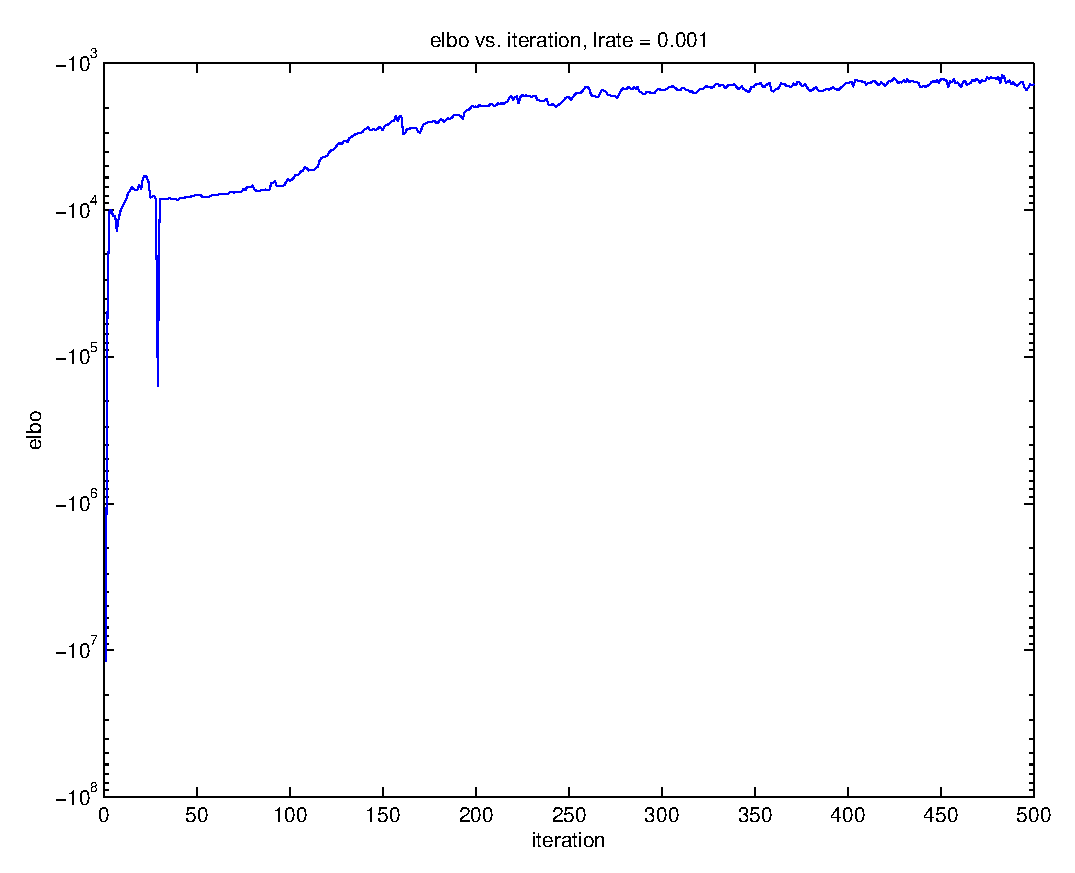
\includegraphics[scale=0.3]{figures/func1-svi-lrate1e-03-bound.eps} &
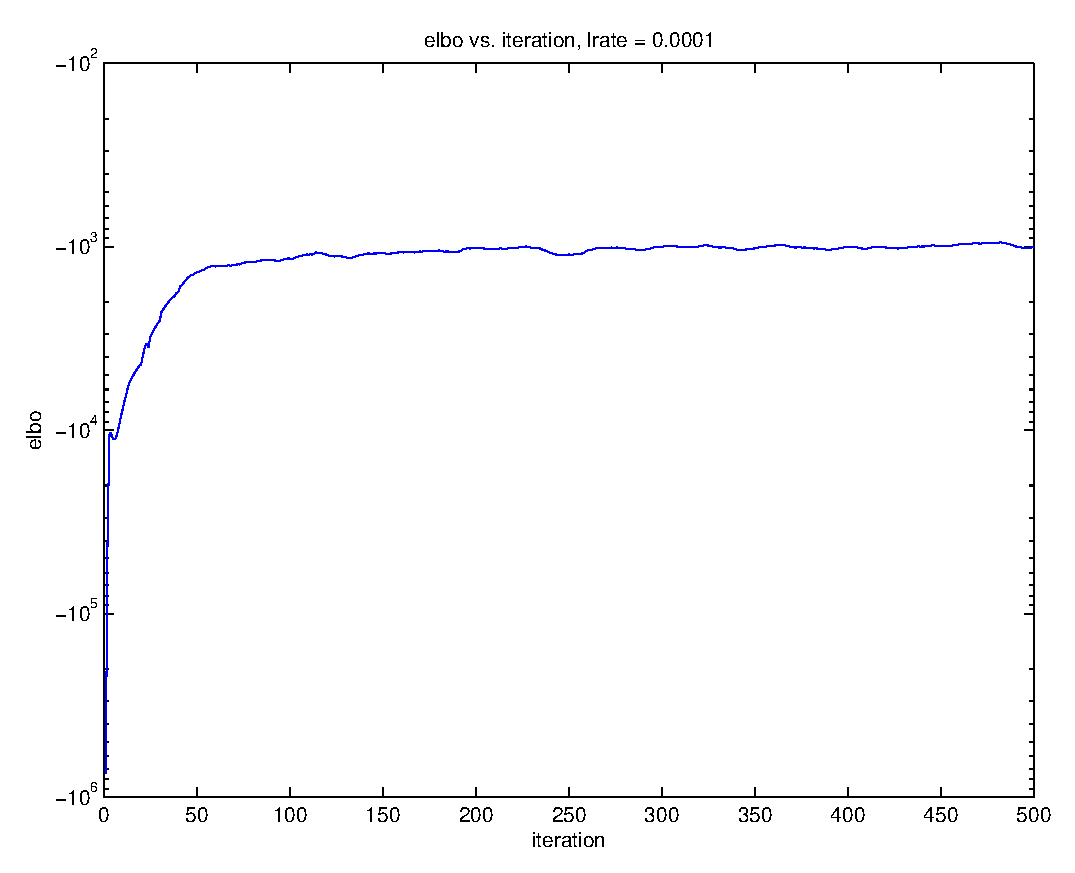
\includegraphics[scale=0.3]{figures/func1-svi-lrate1e-04-bound.eps} &
\includegraphics[scale=0.3]{figures/func1-svi-lrate1e-05-bound.eps} \\ 
(a) learn rate = $1e{-3}$ & (b) learn rate = $1e{-4}$ & (c) learn rate = $1e{-5}$ \\
\multicolumn{3}{c}{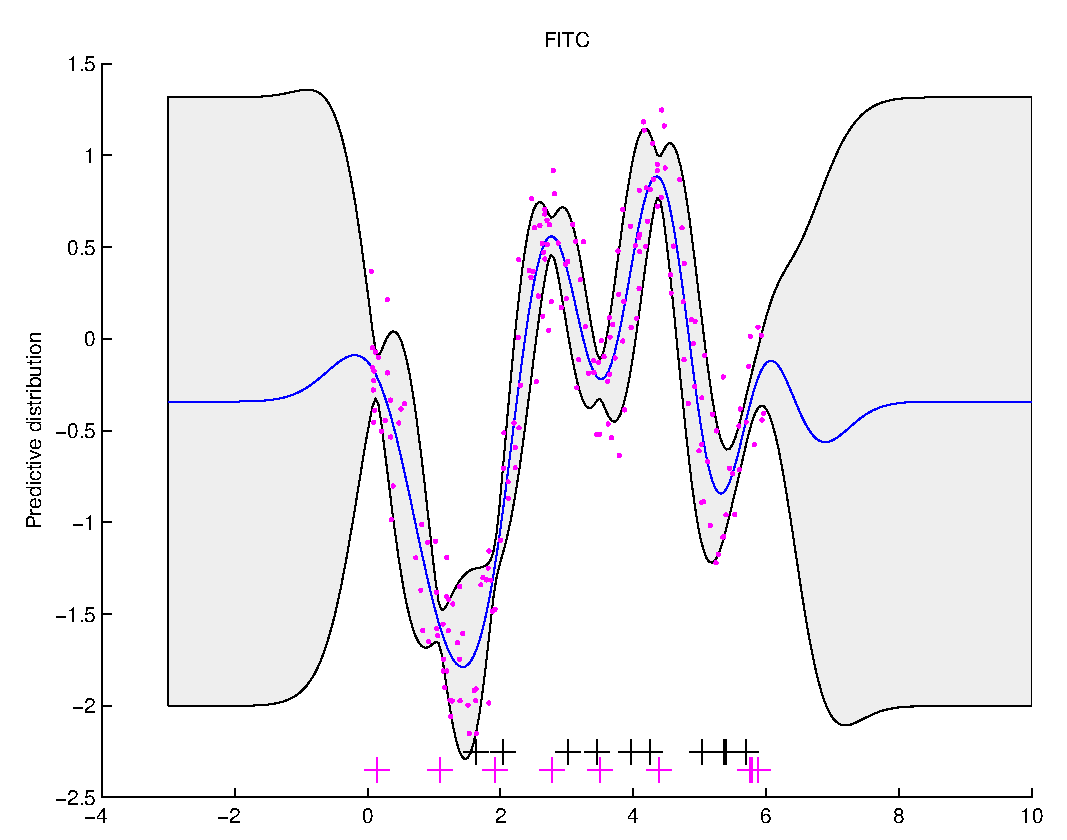
\includegraphics[scale=0.4]{figures/func1-fitc.eps}}
\end{tabular}
\caption{Predictive distributions and learned inducing inputs by GPSVI and FITC for the first function. Top row: GPSVI with different learning rates (the rates decreases from left to right). Bottom row: FITC. Magenta dots : training points. Solid blue line: predictive mean. Grey-shaded area and solid black lines: two standard deviations of the predictive distributions. Black (+) crosses: initial locations of inducing inputs. Magenta (+) crosses: learned locations of inducing inputs.  Middle row: the evidence lower bound of gpsvi vs. iteration.}
\label{fig1}
\end{figure*}

\begin{figure*}
\centering
\begin{tabular}{ccc}
\includegraphics[scale=0.3]{figures/func2-svi-lrate1e-03.eps} &
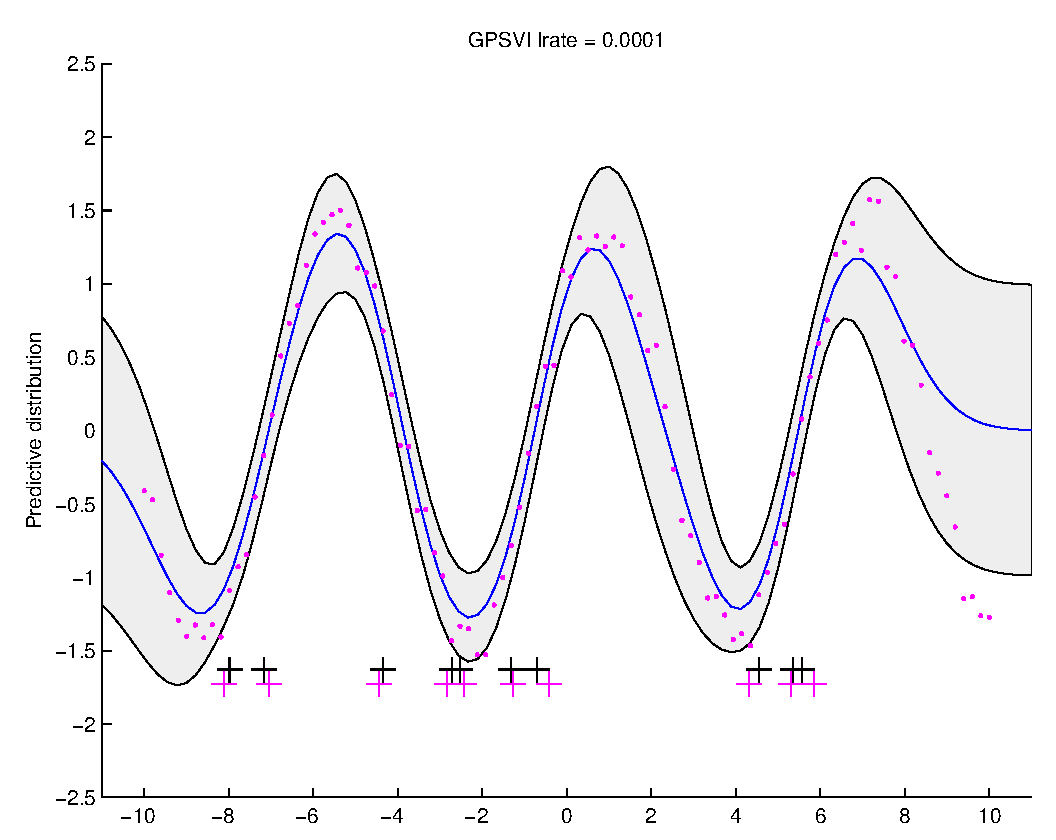
\includegraphics[scale=0.3]{figures/func2-svi-lrate1e-04.eps} &
\includegraphics[scale=0.3]{figures/func2-svi-lrate1e-05.eps} \\
\includegraphics[scale=0.3]{figures/func2-svi-lrate1e-03-bound.eps} &
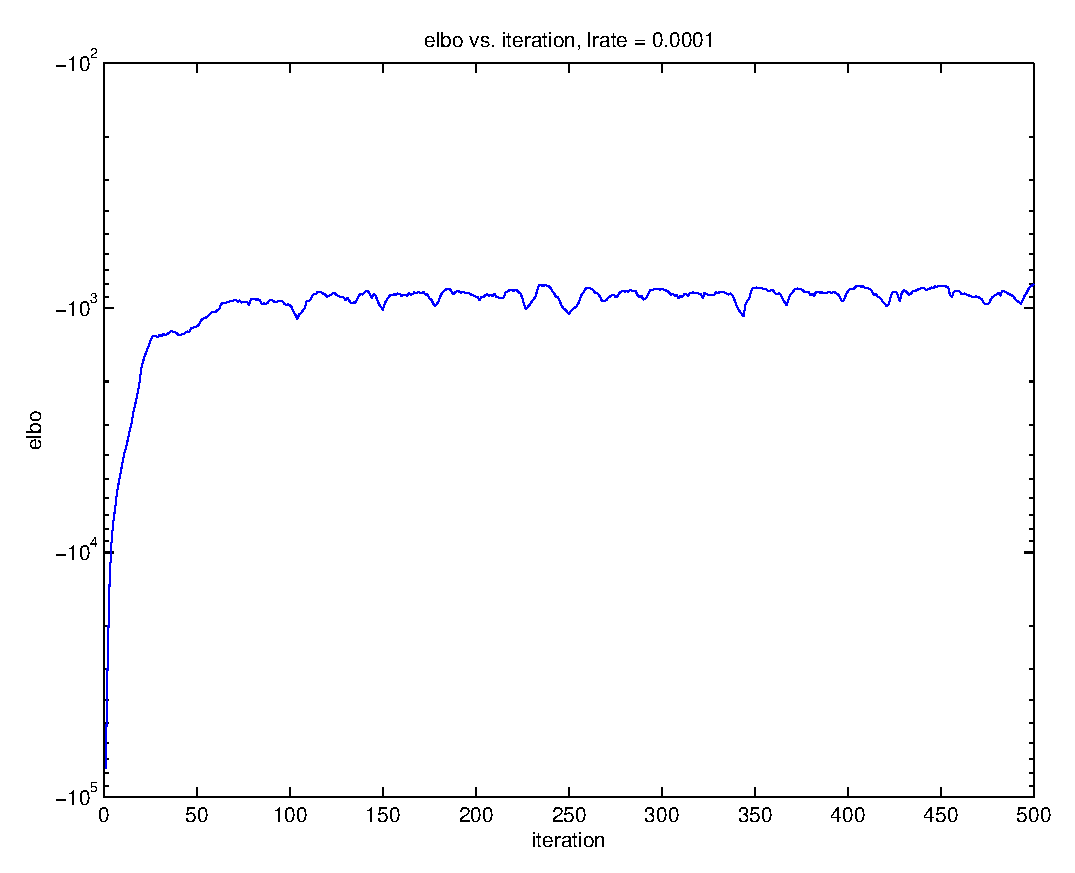
\includegraphics[scale=0.3]{figures/func2-svi-lrate1e-04-bound.eps} &
\includegraphics[scale=0.3]{figures/func2-svi-lrate1e-05-bound.eps} \\ 
(a) learn rate = $1e{-3}$ & (b) learn rate = $1e{-4}$ & (c) learn rate = $1e{-5}$ \\
\multicolumn{3}{c}{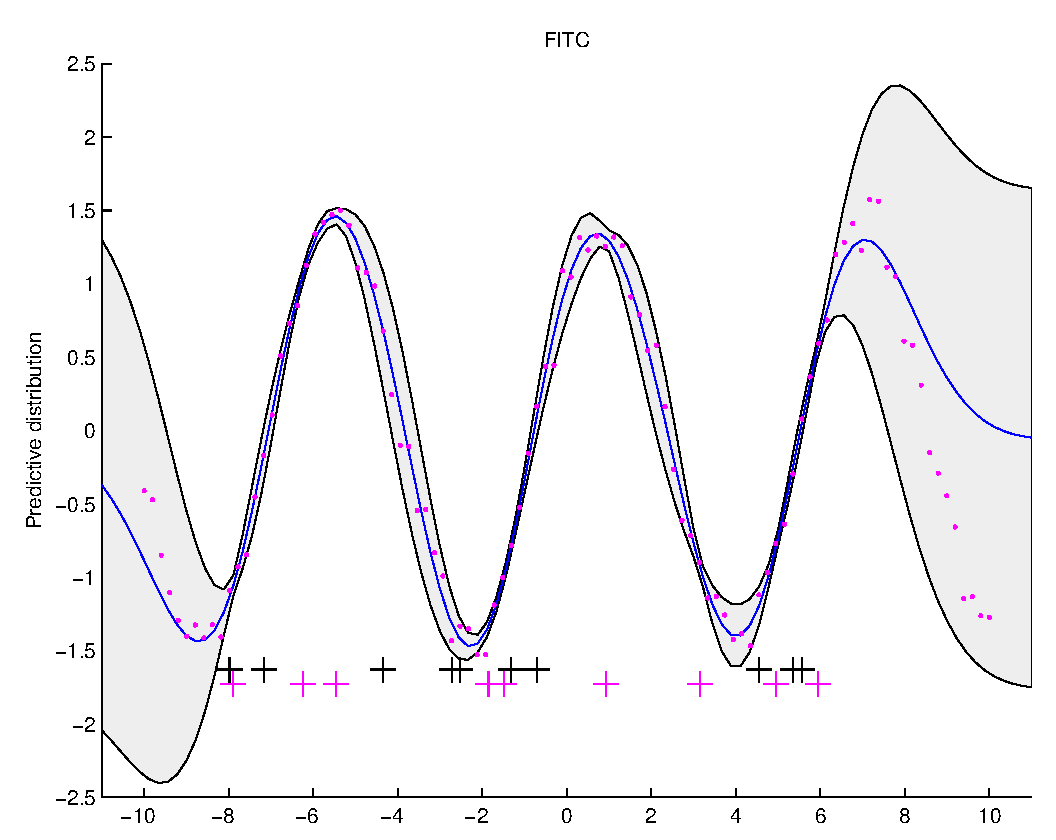
\includegraphics[scale=0.4]{figures/func2-fitc.eps}}
\end{tabular}
\caption{Predictive distributions and learned inducing inputs by GPSVI and FITC for the second function. The legends are same as in Figure 1.}
\label{fig2}
\end{figure*}

\begin{figure*}
\centering
\begin{tabular}{ccc}
\includegraphics[scale=0.3]{figures/func3-svi-lrate1e-03.eps} &
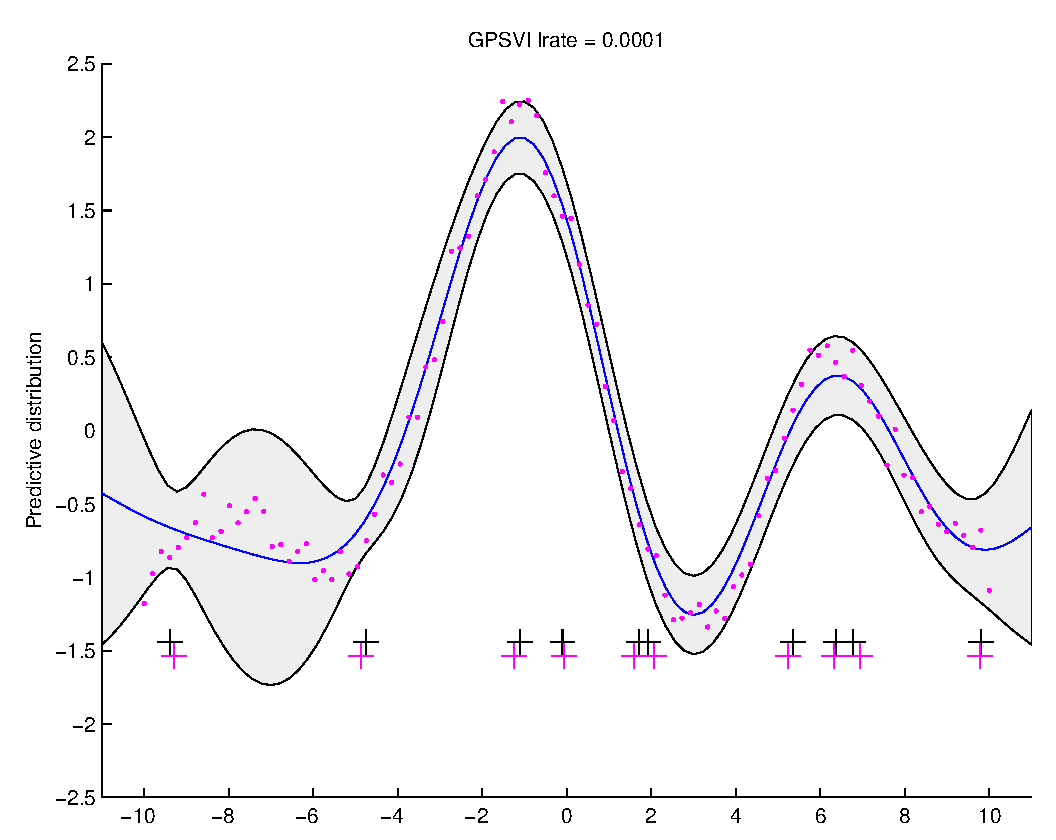
\includegraphics[scale=0.3]{figures/func3-svi-lrate1e-04.eps} &
\includegraphics[scale=0.3]{figures/func3-svi-lrate1e-05.eps} \\
\includegraphics[scale=0.3]{figures/func3-svi-lrate1e-03-bound.eps} &
\includegraphics[scale=0.3]{figures/func3-svi-lrate1e-04-bound.eps} &
\includegraphics[scale=0.3]{figures/func3-svi-lrate1e-05-bound.eps} \\ 
(a) learn rate = $1e{-3}$ & (b) learn rate = $1e{-4}$ & (c) learn rate = $1e{-5}$ \\
\multicolumn{3}{c}{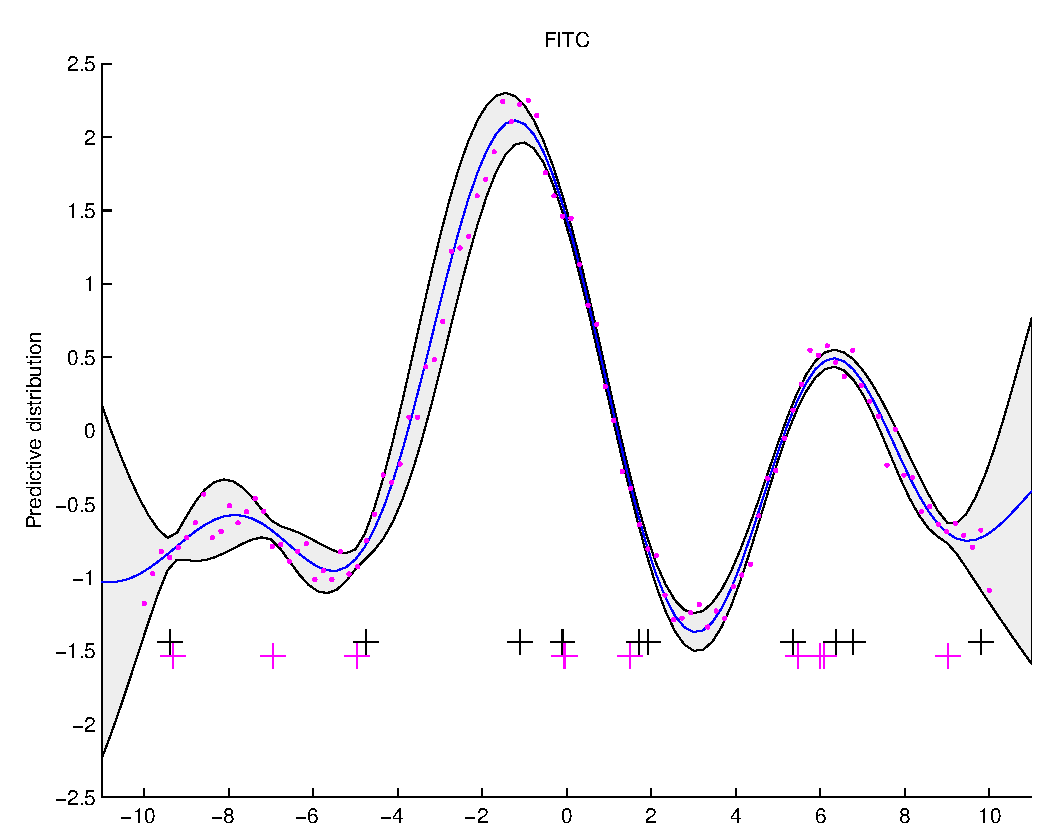
\includegraphics[scale=0.4]{figures/func3-fitc.eps}}
\end{tabular}
\caption{Predictive distributions and learned inducing inputs by GPSVI and FITC for the third function. The legends are same as in Figure 1.}
\label{fig3}
\end{figure*}

\end{document}
